%%%%%%%%%%%%%%%%%%%%%%%%%%%%%%%%%%%%%%%%%
% Twenty Seconds Resume/CV
% LaTeX Template
% Version 1.0 (14/7/16)
%
% This template has been downloaded from:
% http://www.LaTeXTemplates.com
%
% Original author:
% Carmine Spagnuolo (cspagnuolo@unisa.it) with major modifications by 
% Vel (vel@LaTeXTemplates.com) and Harsh Gadgil
%
% License:
% The MIT License (see included LICENSE file)
%
%%%%%%%%%%%%%%%%%%%%%%%%%%%%%%%%%%%%%%%%%

%----------------------------------------------------------------------------------------
%    PACKAGES AND OTHER DOCUMENT CONFIGURATIONS
%----------------------------------------------------------------------------------------

\def\zh_CN_CV{1}

%\documentclass[letterpaper]{twentysecondcv} % a4paper for A4
\documentclass[utf8]{twentysecondcv} % a4paper for A4
%\usepackage[utf8]{inputenc}

% Command for printing skill progress bars
\newcommand\skills{ 
~
    \smartdiagram[bubble diagram]{
        \textbf{Self-motivated}\\\textbf{Dev},
        \textbf{Relational/}\\\textbf{Document}\\\textbf{DB},
        %\textbf{~~~~OOP~~~~~},        
        \textbf{Latex/}\\\textbf{Markdown},
        \textbf{Web}\\\textbf{Stuff},
        \textbf{Machine}\\\textbf{Learning},
        \textbf{Deep}\\\textbf{Learning},
        \textbf{Hardware}\\\textbf{Programming},
        \textbf{Computer}\\\textbf{Vision}
    }
}

\interests{{Functional Programming/4.5},{ML DL/5},{Software Engineering/6},{Computer Vision/6}}

%----------------------------------------------------------------------------------------
%     PERSONAL INFORMATION
%----------------------------------------------------------------------------------------

% If you don't need one or more of the below, just remove the content leaving the command, e.g. \cvnumberphone{}



\cvname{{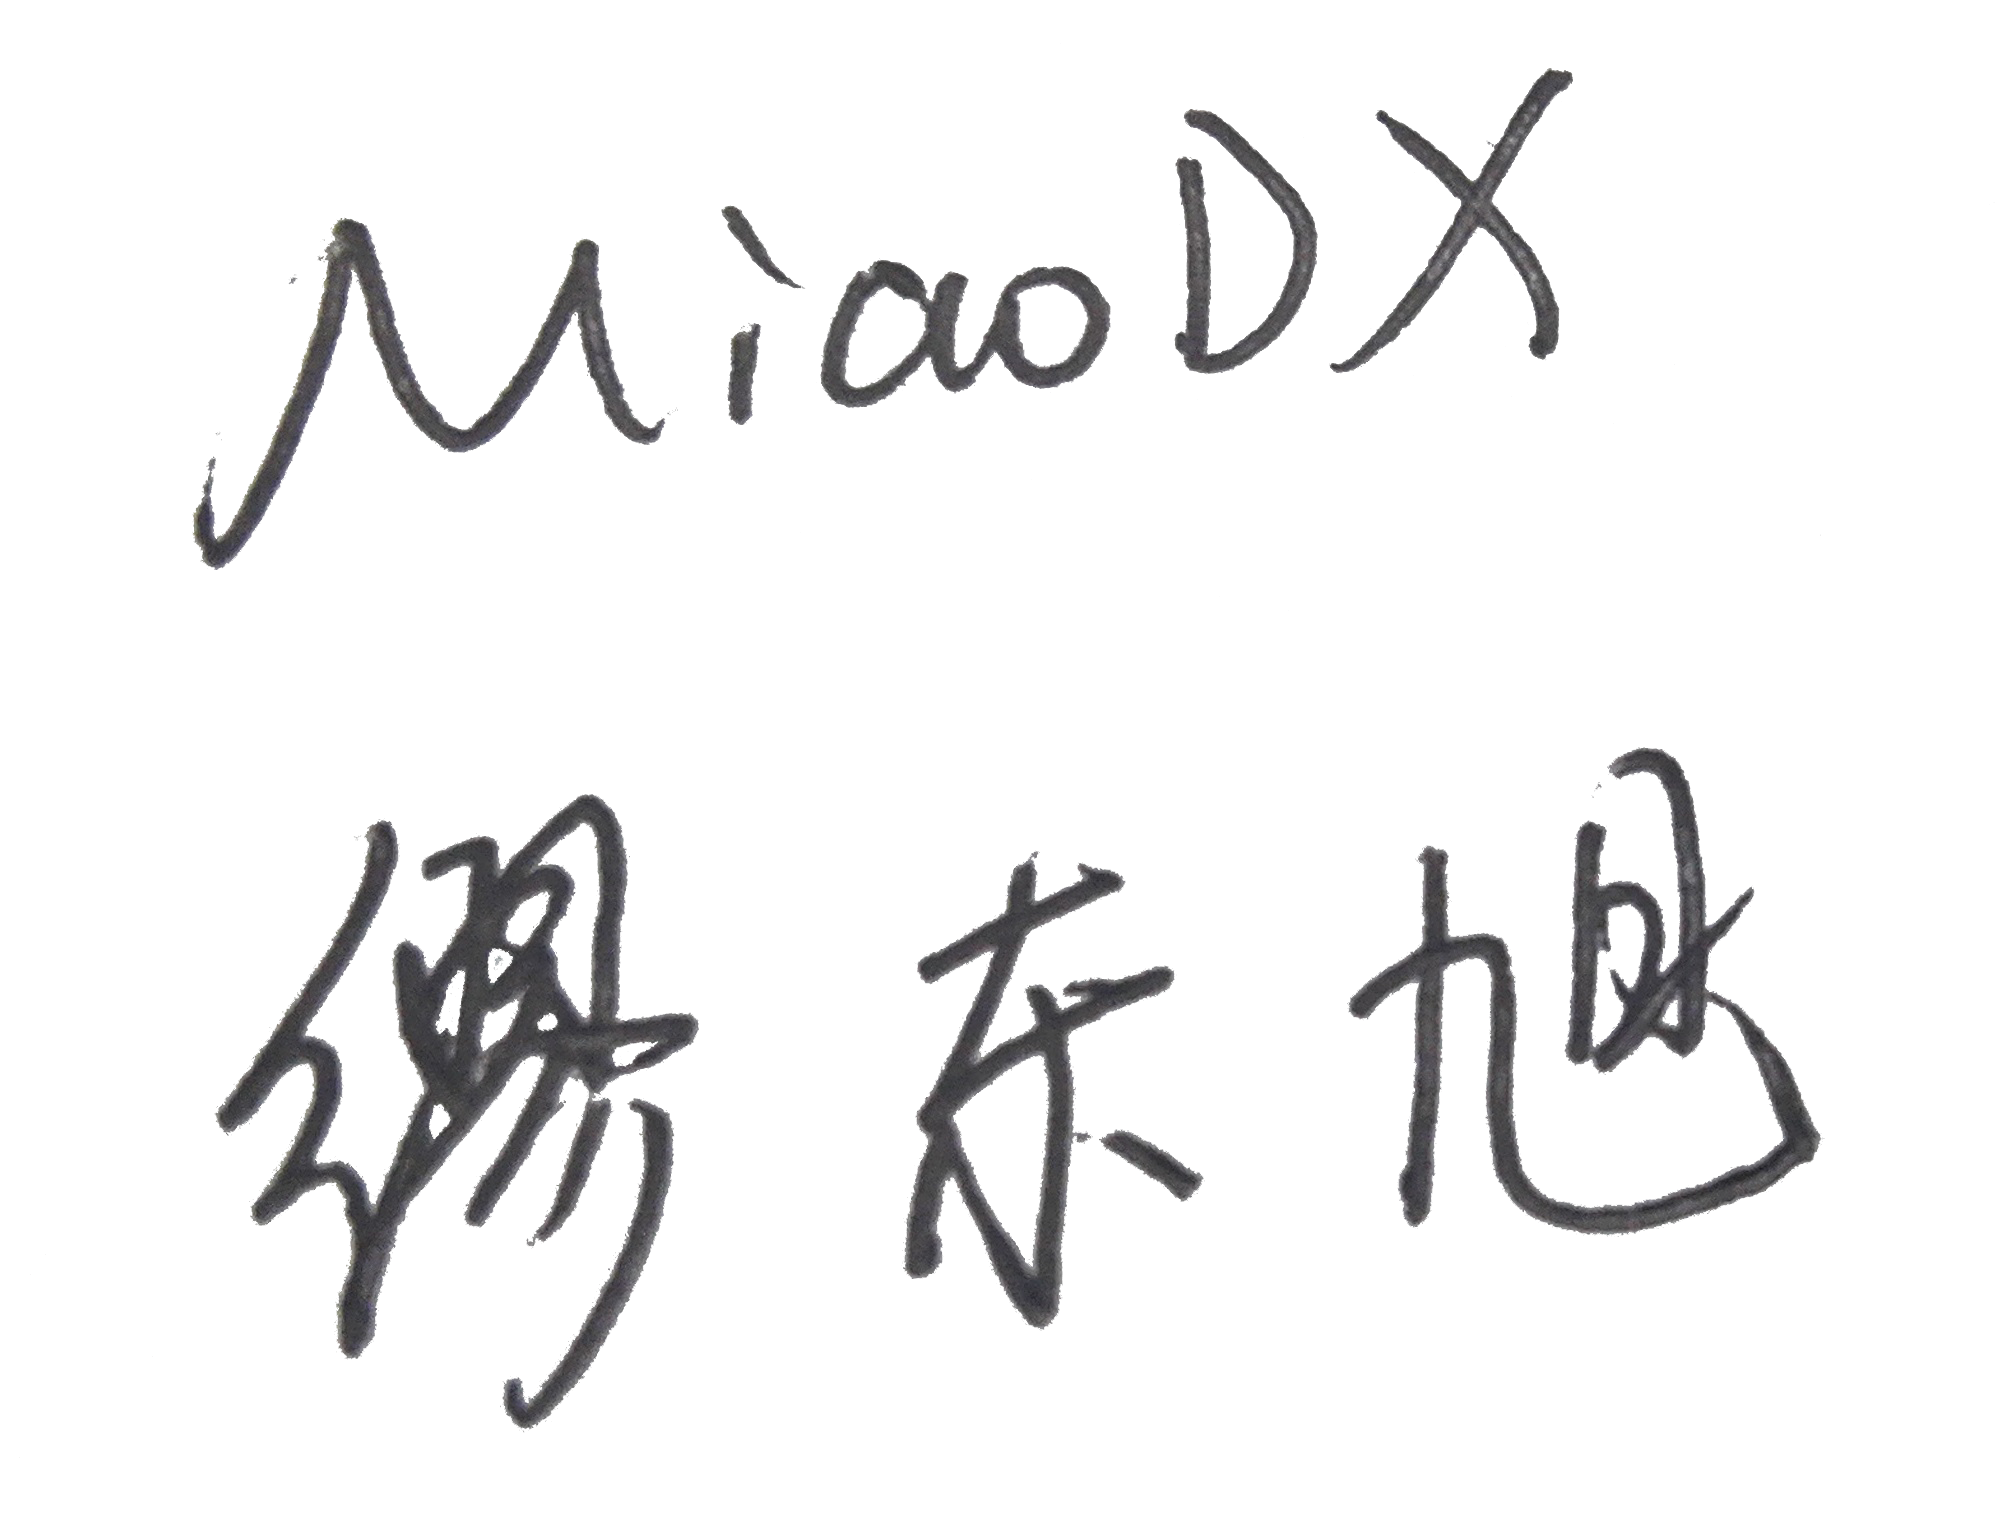
\includegraphics[scale=0.04]{img/miaodx_name.png}}} % Your name
\cvjobtitle{ Graduate Student, \\ Self-motivated Developer} % Job title/career

%\cvlinkedin{https://linkedin.com/in/miaodx}
\cvgithub{https://github.com/MiaoDX}
\cvnumberphone{+86 13502009660} % Phone number
\cvsite{https://miaodx.github.io/} % Personal website
\cvmail{miaodx@tju.edu.cn} % Email address

%----------------------------------------------------------------------------------------

\begin{document}

\makeprofile % Print the sidebar

%----------------------------------------------------------------------------------------
%     EDUCATION
%----------------------------------------------------------------------------------------
\section{教育背景}

\begin{twenty} % Environment for a list with descriptions
    \twentyitem
        %{Expected \\ Dec 2016}
        {2016 - Now}
        {硕士\ 软件工程}
        {\href{http://tju.edu.cn/}{天津大学}}
        {计算机视觉}
        {}
    \twentyitem
        {2012 - 2016}
        {学士\ 软件工程}
        {\href{http://www.xidian.edu.cn/}{西安电子科技大学}}
        {}
        {}
    %\twentyitem{<dates>}{<title>}{<organization>}{<location>}{<description>}
\end{twenty}



\section{荣誉奖励}

\begin{twenty}
    \twentyitem
        {2017-2018}
        {校级二等奖学金}
        {天津大学}
        {}
        {}
    \twentyitem
        {2016-2017}
        {校级一等奖学金}
        {}
        {}
        {}
    \twentyitem
        {Oct 2016}
        {研究生推免至天津大学软件学院}
        {}
        {}
        {}
    \twentyitem
        {2014-2015}
        {国家励志奖学金}
        {西安电子科技大学}
        {}
        {}
    \twentyitem
        {2014CUMCM}
        {全国大学生数学建模竞赛,陕西赛区二等奖}
        {}
        {}
        {}
    \twentyitem
        {2013-2014}  
        {校级二等奖学金}
        {}
        {}
        {}
    \twentyitem        
        {2012-2013}
        {校级一等奖学金}
        {}
        {}
        {}        
\end{twenty}

\section{会议文章}

\begin{twenty}
    \twentyitem
        {Jan 2018}
        {ICASSP 2018, CCF-B 类会议接收}
        {}
        {}
        {ACTIVE CAMERA RELOCALIZATION WITH RGBD CAMERA
FROM A SINGLE 2D IMAGE (Camera ready, 第一作者)}
\end{twenty}

\section{项目经验}
\begin{twenty}

    \twentyitem
        {}
        {列举部分近期项目,更多的请访问 github 主页}
        {\href{https://github.com/MiaoDX/}{github.com/MiaoDX}}
        {}
        {}
          
    \twentyitem
    {Jan 2018 - \\ Present}
    {ICRA 2018 DJI ROBOMASTER AI CHALLENGE}
    {}
    {}
    {ICRA 2018 DJI RoboMaster 人工智能挑战赛,搭建全自动智能车及完成软硬件控制,与大疆官方的 AI 智能车进行对抗。主要负责视觉算法,物体识别、跟踪及部分决策模块(正在进行项目)。}              
          

    \twentyitem
    {Mar 2016 - \\ Present}
    {主动相机位姿重定位}
    {}
    {}
    {主动地将相机位姿重定位到参考位置是机器人学与计算机视觉一基础研究领域,研究生实验室工作主要基于此项目。本科毕设便是改善与提升实验室现有软硬件平台,今年通过利用 RGBD 相机获取的深度信息重定位相机使得我成功发表了 CCF-B 类会议文章。}
          
    \twentyitem
        {Virtual Env \\ DL}
        {Unrealcv 与深度学习结合 (Faster-RCNN)}
        {\href{https://github.com/MiaoDX/unrealcv_examples/}{Unrealcv with DL}}
        {}
        {将一 faster rcnn 的 TensorFlow 实现 (\href{https://github.com/smallcorgi/Faster-RCNN\_TF}{smallcorgi/Faster-RCNN\_TF}) 配合 \href{https://github.com/unrealcv/unrealcv}{unrealcv} 结合到基于 Unreal4 游戏引擎的虚拟仿真环境上,探究通过合成数据来提升现有深度学习实现的可能性。}
                 
    \twentyitem
        {Python \\ RL}
        {PacMan capture the flag 增强学习应用到吃豆人游戏}
        {\href{https://github.com/MiaoDX/hand_in_homework/tree/master/Advanced\_AI/}{PacMan with RL}}
        {}
        {整理了增强学习的一些基础知识,并将其应用到吃豆人游戏当中,在高级人工智能结课比赛中取得较好成绩。}
   
    \twentyitem
        {OpenCV}
        {Notes on OpenCV}
        {\href{https://github.com/MiaoDX/opencv\_projects/}{opencv\_notes}}
        {}
        {使用 OpenCV 过程中的一些记录、示例代码以及技巧总结。}

\end{twenty}



\begin{twenty}

    \twentyitem
        {Python \\ ML}
        {利用 scikit-learn 库处理 UCI Adult 数据集}
        {\href{https://github.com/MiaoDX/scikit\_learning/}{scikit\_learning}}
        {}
		{基于人口调查结果,使用 scikit-learn 机器学习库来预测收入是否超过 \$50K/yr,这是一典型的分类问题。在课程设计阶段在班级内部取得最好结果(仅使用 sklearn 库分类精度在测试集上达到 85\%-86\% 的精度)。}        
     	
	

        
    \twentyitem
        {Java \\ BP}
        {使用 Java 实现反向传播算法}
        {\href{https://github.com/MiaoDX/bp_java}{bp\_java}}
        {}                
        {在使用流行的开源 ML(\/DL) 库前,我认为能够先从头实现一些基本的组件是很重要的。这样会对 NN 有更多的理论认识并且知道其运算机理,远比将其视为黑盒要好得多。}

    \twentyitem
        {Node.js \\ mongodb}
        {考勤管理系统}
        {\href{https://github.com/SEAPC2016/attendance}{attendance system}}
        {}
        {课程设计,使用 Node.js, mongodb 以及 Jade 为一(模拟)公司实现了基于 RESTful 接口的考勤管理系统。公司成员可以经由本系统申请休假并等待上级批准,同时可以查询由系统整理得到的历史统计数据。}

        
%    \twentyitem
%        {Baidu Map API  \\ D3.js}
%        {Display churches in Tianjin}
%        {\href{https://github.com/MiaoDX/baidu\_map\_church}{baidu\_map\_church}}    
%        {}
%        {Course project of Visual Analysis class, since I really love the architecture of old churches, so I use Baidu Map API to get all churches' locations in Tianjin and display them with D3.js.}    


\end{twenty}


\section{工作经验}

%\begin{twenty}
%

%


%   
%

%
%
%   
%
%
%    
%    
%\end{twenty}

\begin{twenty}

\twentyitem
    {June 2017 - \\ Now}
    {TJU RM 成员}
    {天津大学}
    {}
   	{天津大学大疆 Robomaster 团队成员,算法组,负责将计算机视觉及深度学习算法用于物体识别、跟踪以及决策。}

\twentyitem
    {Feb 2017 - \\ July 2017}
    {研究生期间助教}
	{}
    {}
    {大一新生程序设计实践 I 助教,教授为外籍老师,课程全英文教学。负责问题解答,作业及考试批改。}


\twentyitem
    {Feb 2017 - \\ May 2017}
    {Python101 课程}
    {\href{https://github.com/MiaoDX/python101}{MiaoDX/python101}}
    {}
    {为几位已申请到国外高校的金融专业准硕士/博士教授 python 基础,课程为期一月,传播知识的同时也加深了自己对 python 的掌握。}
    
\twentyitem
    {2013 暑期}
    {志愿者教师}
    {\href{http://blog.sina.com.cn/xiaanedu}{陕西 滴水行动}}
    {}
    {与队友一起在陕西省铜川市一山村小学做为期 18 天的志愿教学,活动由陕西青年与环境互助网络组织进行。在此过程中与当地学生一起生活成长,介绍了不少科学知识。}    
    
\twentyitem
    {Sep 2012 - \\ Sep 2013}
    {本科社团活动}
    {\href{http://www.xidian.edu.cn/}{西安电子科技大学}}
    {}
    {校青年志愿者组织及勤工助学中心成员。}

    
\end{twenty}



\section{其他信息}

\begin{twenty} % Environment for a list with descriptions
    
\twentyitem
    {}
    {}
    {}
    {}
    {        
        {\begin{itemize}
            \item Passed CET-6 (460), English as working language
            \item 阅读\ 拳击\ 跑步\ 骑行     
        \end{itemize}
         }
    }    
        
    %\twentyitem{<dates>}{<title>}{<location>}{<description>}
\end{twenty}

\end{document} 
